\section{Aufbau und Durchführung}
\label{sec:Durchführung}

\subsection{Aufbau und Durchführung um das Abbildungsgesetz und die Linsengleichung zu verifizieren}
\label{sec:Versuchsaufbau}
Um das Abbildungsgesetz und die Linsengleichung zu verifizieren wird eine optische Bank benötigt, an deren einem Ende sich eine Halogenlampe befindet und am anderen Ende ein Schirm. Dazwischen wird ein Gegenstand "Perl L" und eine Sammellinse mit bekannter Brennweite $f$ positioniert. Der Gegenstand steht zwischen der Halogenlampe und der Sammellinse. Die Position des Schims wird solange geändert bis der Gegenstand als scharfes Bild erscheint. Die Gegenstandsweite $g$ wird dabei nicht verändert. Nachdem das Wertepaar ($g_\text{i}, b_\text{i}$) aufgeschrieben wurde, wird die Versuchsreihe mit neun weiteren Gegenstandsweiten fortgesetzt. Zum Schluss werden alle Wertepaare in ein Koordinatensystem eingezeichnet. Die Gegenstandsweiten $g_\text{i}$ werden auf die x-Achse aufgetragen und die Bildweiten $b_\text{i}$ auf die y-Achse. Nun werden die einzelnen Wertepaare durch Geraden verbunden und der Schnittpunkt $A$ aller Geraden entspricht der Brennweite $f$ (siehe Abbildung \eqref{fig:Brennweite}).

\begin{figure}[H]
  \centering
  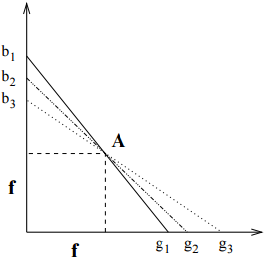
\includegraphics[height=5cm]{picture/Brennweite}
  \caption{Die Wertepaare ($g_\text{i}, b_\text{i}$)aufgetragen. \cite[3]{sample}}
  \label{fig:Brennweite}
\end{figure}

\subsection{Bestimmung der Brennweite einer Linse nach dem Bessel-Verfahren}
Der Versuchsaufbau zur Bestimmung der Brennweite einer Linse nach dem Bessel-Verfahren ist identisch mit dem Aufbau aus dem Kapitel \eqref{sec:Versuchsaufbau}. \\
Zu Beginn wird ein fester Abstand $e$ zwischen dem Gegenstand und dem Schirm gewählt und die Linse an die Halogenlampe gestellt. Nun soll die Linse in Richtung des Schirms bewegt werden, bis ein scharfes Bild zu erkennen ist und es wird das Wertepaar ($g_1, b_1$) aufgeschrieben. Wenn bei gleichem Versuchsaufbau die Linse weiter in Richtung des Schirms bewegt wird, ergibt sich ein zweites Mal ein scharfes Bild. Das Wertepaar wird als ($g_2, b_2$) notiert und die Versuchsreihe für neun weitere Abstände $e$ wiederholt. \\
Um die chromatische Abberation zu untersuchen, werden für jeweils fünf Abstände $e$, ein roter und ein blauer Filter vor den Gegenstand gesetzt. Die Messung läuft analog zu oben beschriebenen Bessel-Verfahren.

\subsection{Bestimmung der Brennweite eines Linsensystems nach Abbe}
Für diesen Versuchsaufbau werden auf der optischen Bank die Halogenlampe, der Gegenstand, eine Zerstreuungslinse, eine Sammellinse und der Schirm in eben dieser Reihenfolge aufgebaut. Der Abstand zwischen den beiden Linsen muss für die gesamte Messung konstant gehalten werden. Nun wird das Linsensystem verschoben, bis ein scharfes Bild auf dem Schirm zu erkennen ist. Die Bild- und Gegenstandsweiten $b'$ und $g'$ werden zu einem Referenzpunkt $A$ gemessen. Für die Messungen wird der Referenzpunkt $A$ auf die Mittelebene der Sammellinse gelegt. Zusätzlich werden die Bild- und Gegenstandgrößen $B$ und $G$ gemessen. Diese Messung wird für neun weitere Gegenstandsweiten durchgeführt.
